\chapter{Method}
\label{sec:method}



\section{Overview}

\begin{figure}[h]
    \centering
    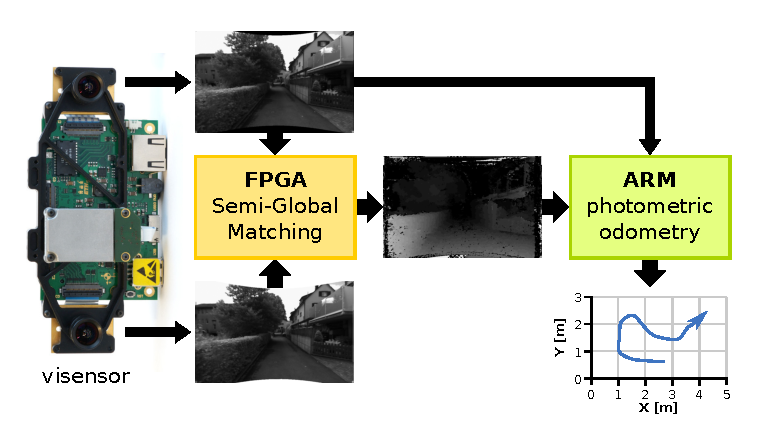
\includegraphics[width=\textwidth]{images/system_overview.pdf}
    \caption{schematic overview of the whole system}
    \label{fig:overview}
\end{figure}


The visensor provides a stream of frames, each of which consists of a stereo
pair of grayscale intensity data \footnote{Grayscale instead of full-color
images are used, because the information gain from colors is offset by the loss
of resolution. However, the approach described here would work similarly
with colored images.}.  A semiglobal stereo matching core developed in
\cite{honegger2014sgmcore} running on the FPGA processes these and produces a
disparity image which assigns every pixel the disparity between the two
cameras. The FPGA also provides a rectified camera image.

This pair of intensity and disparity images is conceptually equivalent to a
three dimensional point-cloud, as we can calculate the distance to the camera
for every pixel from the disparity data. This is in turn makes it possible to
render the point-cloud from an arbitrary perspective, allowing us to look at an
image as if it was recorded from a different angle.

To estimate the ego-motion between two frames we can thus look for a
perspective where the re-rendered image looks the same as the previous frame.
The movement of the virtual camera will then correspond to the actual, physical
movement of the sensor.

The problem is formulized as a minimization problem, by subtracting the
intensities from the previous frame with the intensities of the current frame
sampled at the warped pixel locations. This way, a photometric error is
calculated, measuring the similarity of the warped current frame with the
previous one.

Note that this approach assumes Lambertian reflectance and constant
illumination (also known as photo-consitency), which implies that points should
have the same brightness, regardless of viewing angle.


\section{Warping Pipeline}
\label{sec:warping}

\begin{figure}[h]
    \centering
    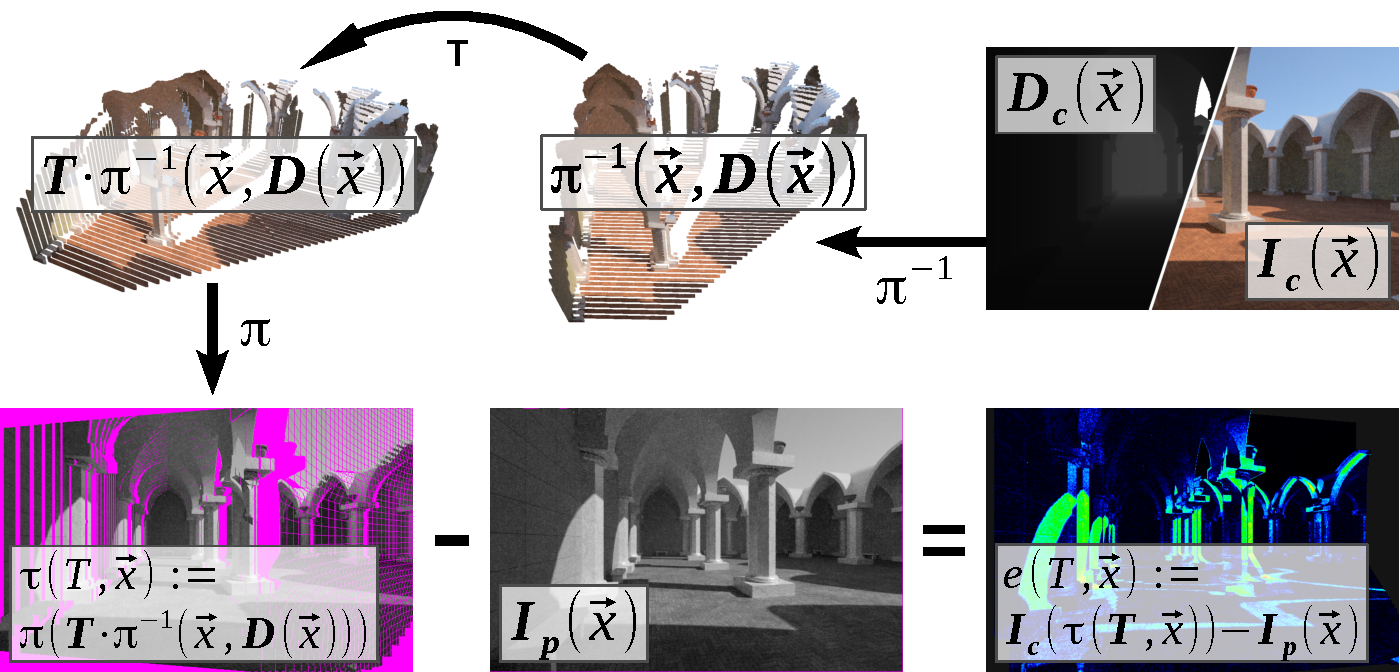
\includegraphics[width=\textwidth]{images/warp_pipeline.pdf}
    \caption{the full warping pipeline (pink pixels are not sampled by any of the warped points)}
    \label{fig:warp_pipeline}
\end{figure}

\begin{figure}
    \begin{minipage}[t]{0.48\textwidth}
        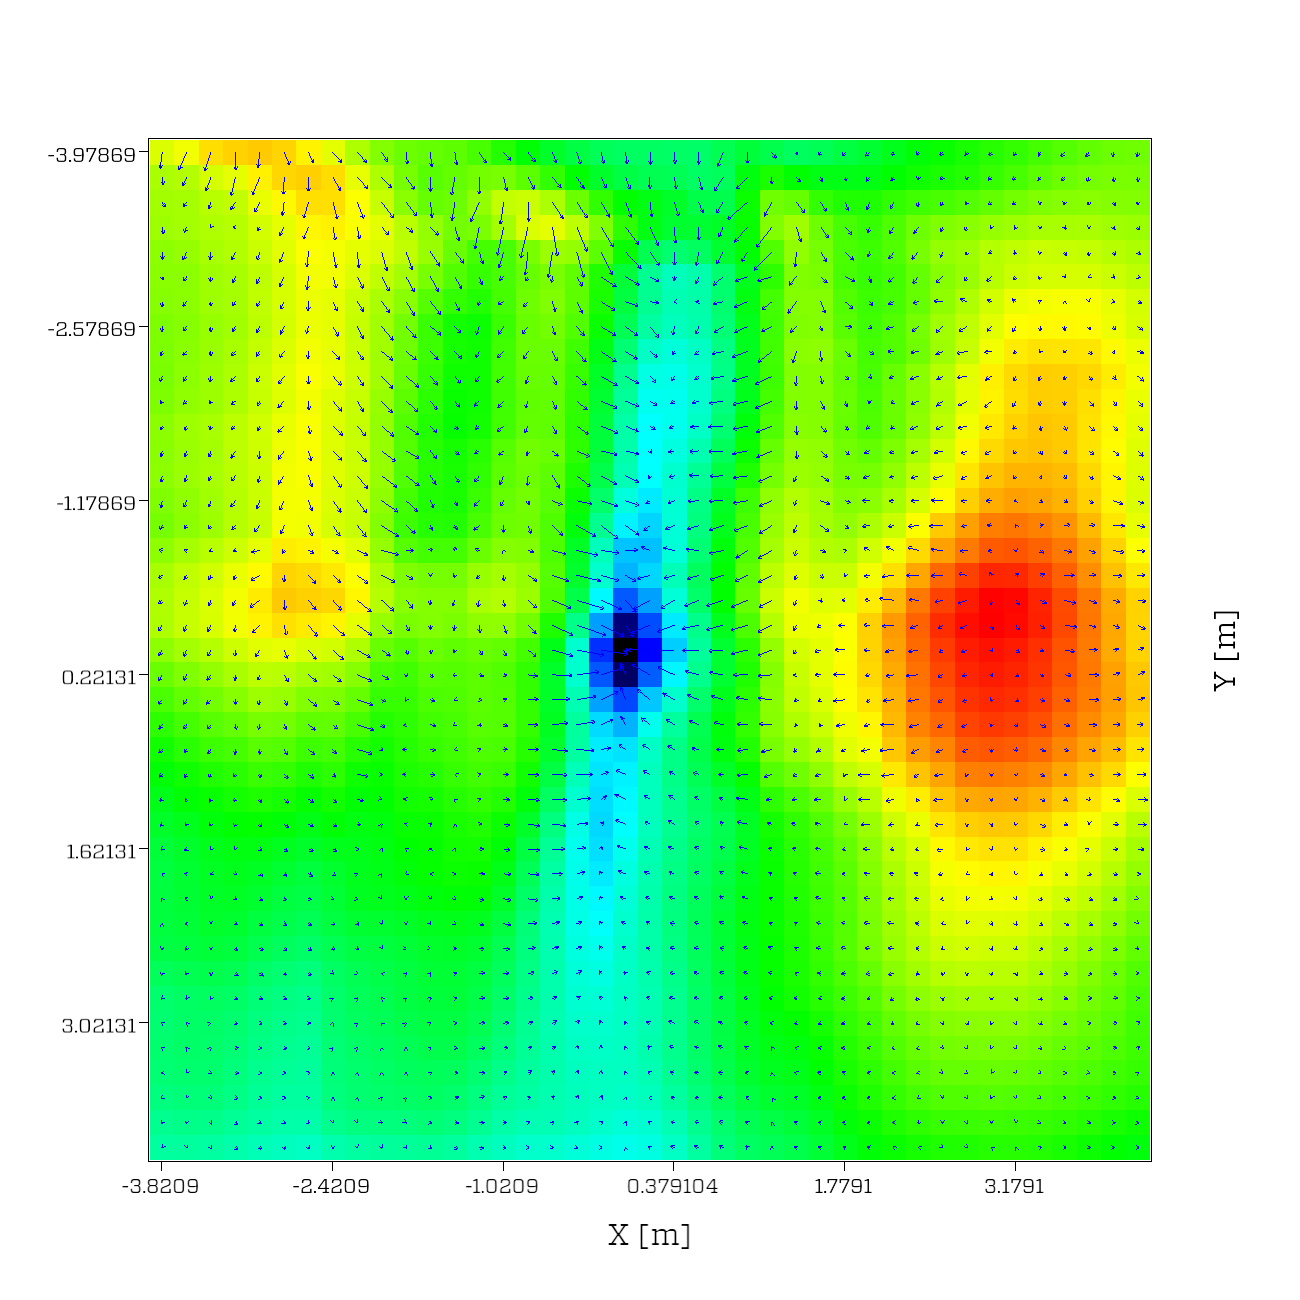
\includegraphics[width = \textwidth]{images/cost_surface/error_xy_4.png}
    \end{minipage}
    \hfill
    \begin{minipage}[t]{0.48\textwidth}
        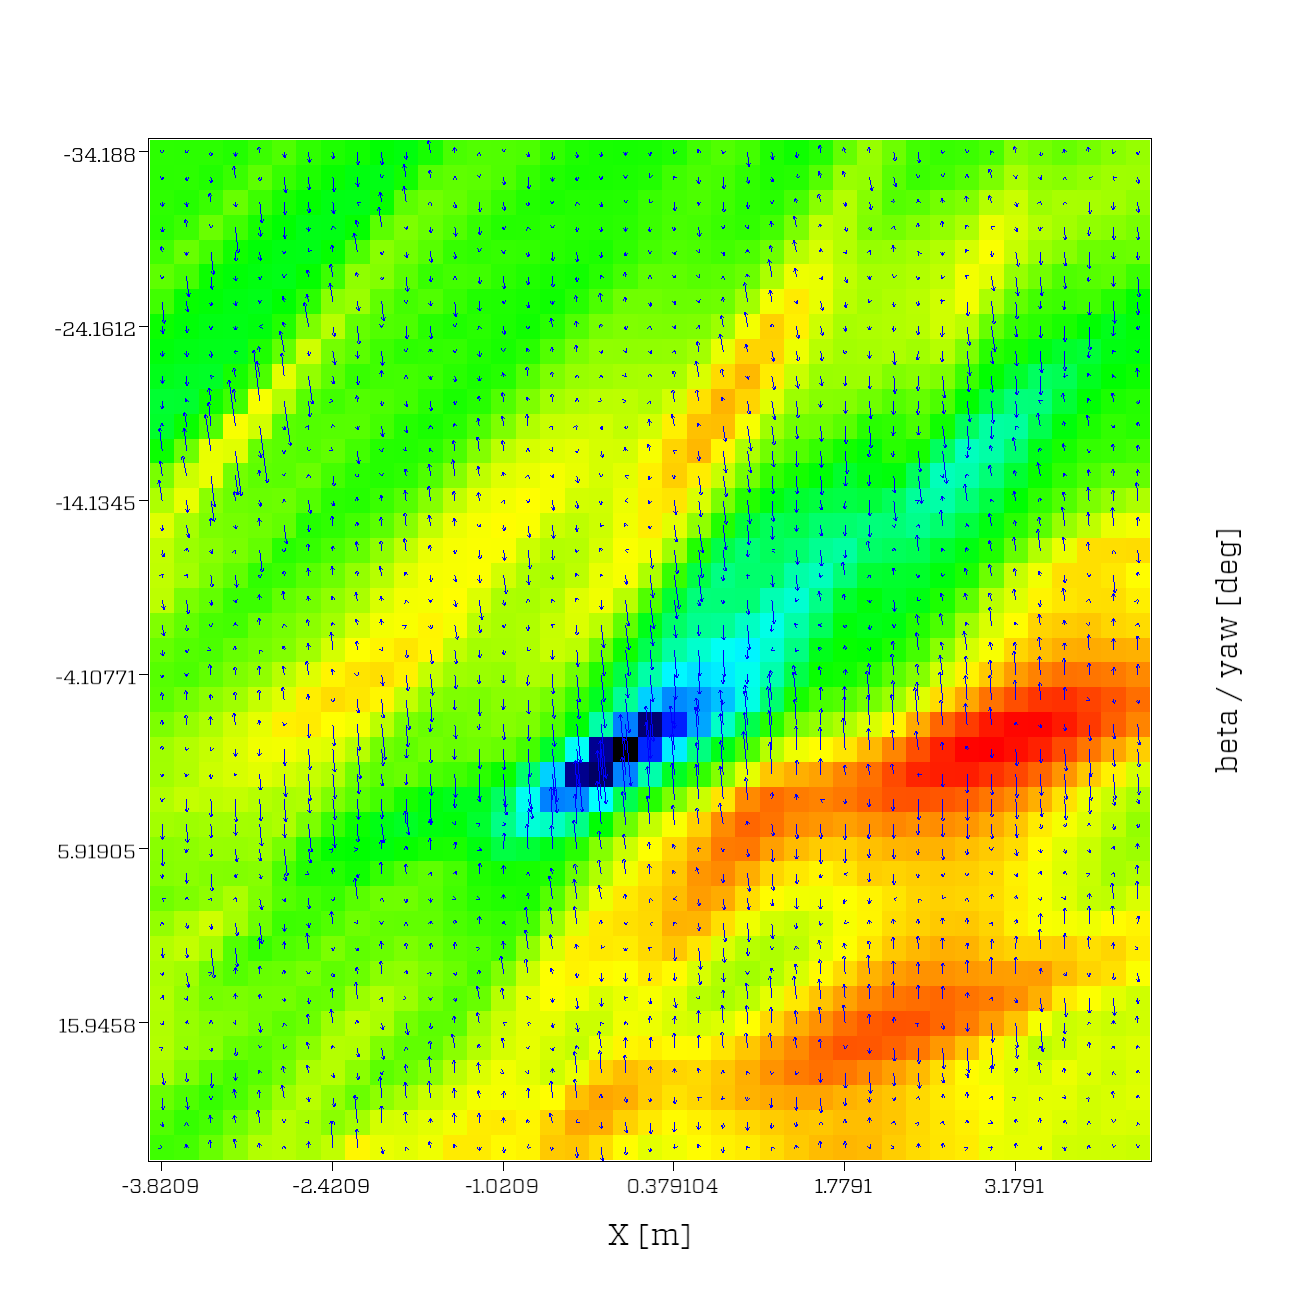
\includegraphics[width = \textwidth]{images/cost_surface/error_xb_4.png}
    \end{minipage}
    \begin{minipage}[t]{0.48\textwidth}
        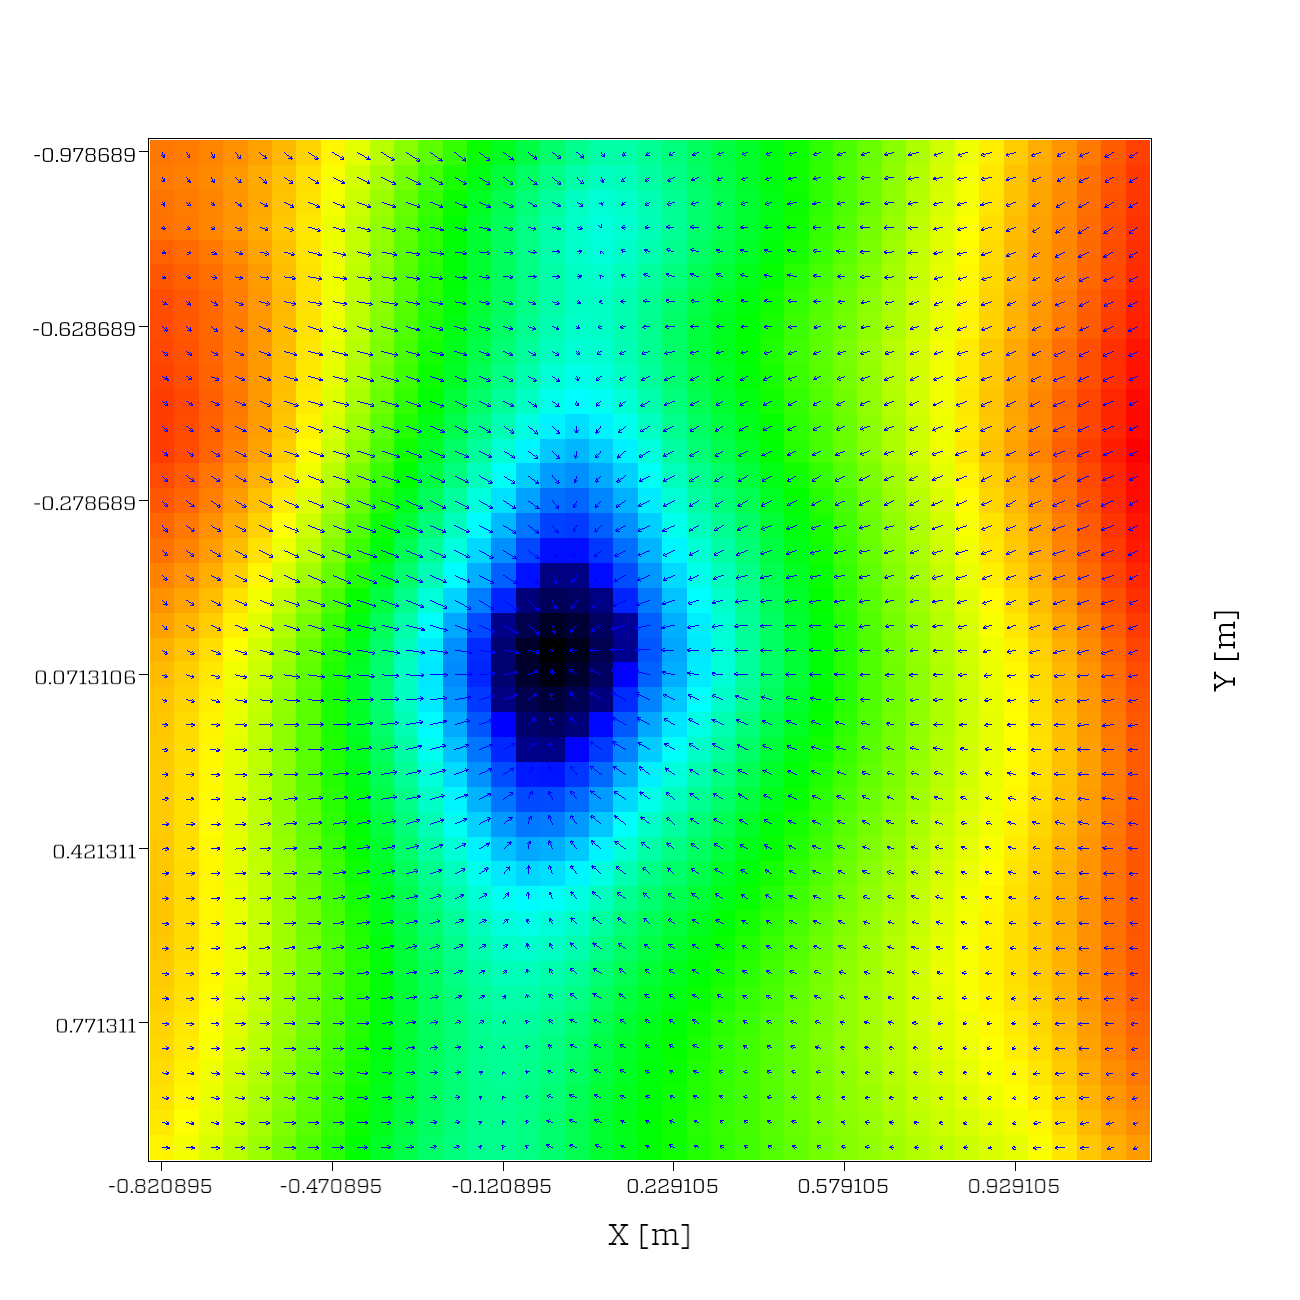
\includegraphics[width = \textwidth]{images/cost_surface/error_xy_1.png}
    \end{minipage}
    \hfill
    \begin{minipage}[t]{0.48\textwidth}
        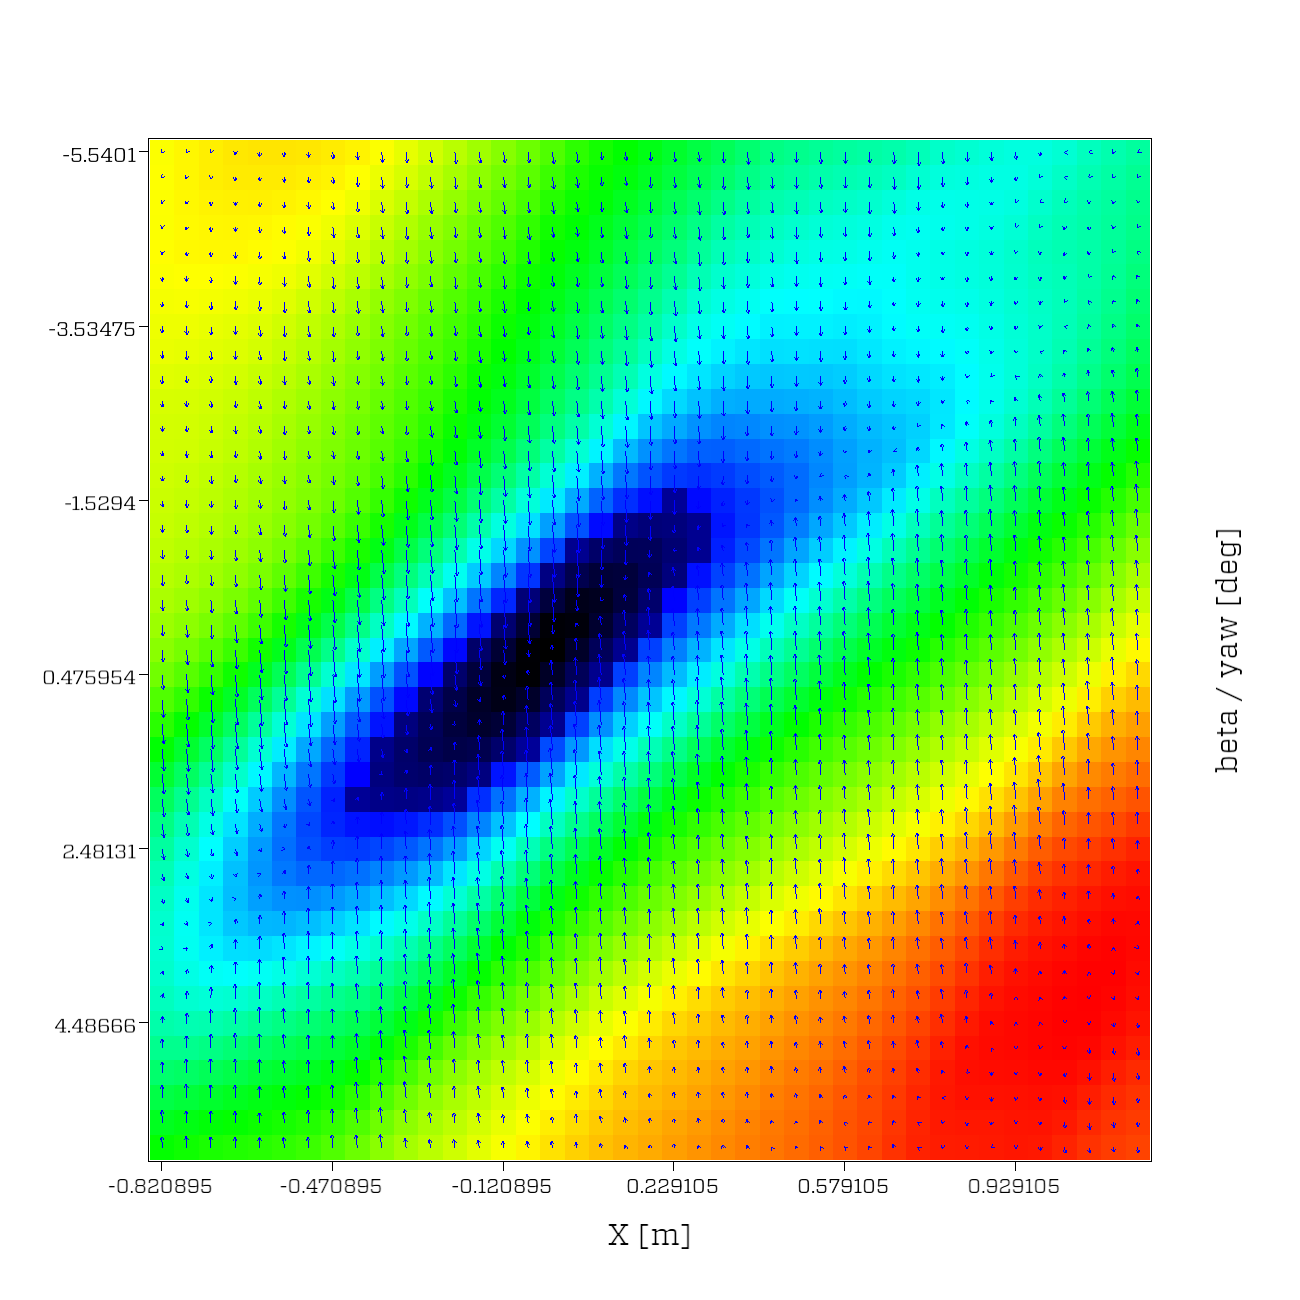
\includegraphics[width = \textwidth]{images/cost_surface/error_xb_1.png}
    \end{minipage}
    \caption{A visualization of the photometric error surface described by $e$
    generated from simulated camera data. Note how displacements of about half
a meter or about \unit[5]{\degree} still lead to the correct minimum. Also
note, that there are many local minima further out.}
    \label{fig:costsurface_big}
\end{figure}

This section closely follows \cite{omaridenseodometry}.

Using an back-projection derived from the standard pinhole camera model, a
point $ \vec{x} = [ x_u  x_v ]^\intercal $ in the camera image plane is be back-projected into a point $
\vec{p_C} \in \mathbb{R}^3 $ (in the current frame of reference; written using
homogeneous coordinates) by using the pixel's disparity value $D_C(\vec{x})$:

\begin{equation}
    \label{eq:backprojection}
    \vec{p_C} = \pi^{-1}(\vec{x}, D_C(\vec{x})) := \frac{b}{D_C(x)}
    \begin{bmatrix}
        x_u - c_u \\
        x_v - c_v \\
        f \\
        1
    \end{bmatrix}
\end{equation}

where $b$ is the stereo baseline, $f$ the focal length and $\vec{c} = [ c_u c_v ]^\intercal$ the principal point of the camera.

This point $\vec{p_C}$ can now be moved into the previous camera frame by translating
and rotating it, by writing the transformation from the previous into the
current camera frame $\vec{T_{PC}}$ as a $4 \times 4$ homogeneous
transformation matrix:

\begin{equation}
    \vec{p_P} = \mat{T_{PC}} \cdot \vec{p_C}
\end{equation}

A point in 3D space can be projected back onto the (now moved) camera image plane:

\begin{equation}
    \label{eq:projection}
    \vec{x'} = \pi(\vec{p_P}) := \frac{f}{p_{z}}
    \begin{bmatrix}
        p_{x} \\
        p_{y} \\
    \end{bmatrix}
    + \vec{c}
\end{equation}

This whole warping operator is summarized in a warping operator $\tau$:

\begin{equation}
    \vec{x'} = \tau(\vec{x}, \vec{T_{PC}}) := \pi( \mat{T_{PC}} \cdot \pi^{-1} (\vec{x}, D_C(\vec{x})))
\end{equation}


\subsection{Representation of Transformation}

While translations are mathematically very straightforward, rotations can be
represented in numerous ways (Euler-angles, quaternions, rotation matrices,
etc.) and proper derivation of the Jacobians can be tricky.

Fortunately, odometry works in a relative fashion without any absolute
orientation and steps are very incremental as photometric odometry cannot
handle more than a few degrees of rotation. This implies we do not have to deal
with gimbal-lock and other mathematical hurdles of working in $SO(3)$. In this
work, Tait-Bryan angles were used, following the ZYX convention (yaw, pitch,
roll).




\section{Minimization}

Using $\tau$, the error between the previous frame and the warped current frame is be defined as:

\begin{equation}
    \label{eq:error}
    e(\vec{x}, \vec{T_{PC}}) := I_P(\tau(\vec{x}, \vec{T_{PC}})) - I_C(\vec{x})
\end{equation}


To estimate the motion between two frames, this photometric error term should
be minimized for every pixel:

\begin{equation}
    \vec{\hat{T}} = \operatornamewithlimits{argmin}_{\vec{T}} \sum_{\vec{x} \in I_p} e(\vec{x}, \vec{T})^2
\end{equation}


This equation can be solved for the estimated motion by applying standard
optimization techniques, for example Gauss-Newton:

\begin{equation}
    \mat{J}^\intercal \mat{J} \Delta \vec{T} = - \mat{J}^\intercal \vec{e(\vec{T})}
\end{equation}

Here, $\mat{J} \in \mathbb{R}^{N \times 6}$ are the stacked Jacobian matrices
and $\vec{e(\vec{T})} \in \mathbb{R}^N$ the vector of the error terms of all
$N$ pixels.  This equation is iteratively solved for the increment $\Delta
\vec{T}$ of the motion estimation after recalculating the error term and
Jacobians from the new estimation.

The Jacobian is derived by applying the chain rule to the photometric error term \ref{eq:error}.
For a single pixel, we get a $1 \times 6$ Jacobian:

\begin{equation}
    \mat{J} := \mat{J_I} \mat{J_{\pi}} \mat{J_T}
\end{equation}

where $\mat{J_I} \in \mathbb{R}^{1 \times 2}$ is the image derivative of the warped previous frame and is
approximated using the image's gradient:

\begin{equation}
    \mat{J_I} := \frac{\partial I_p(\vec{x})} {\partial \vec{x}} \bigg|_{\vec{x} = \tau(\vec{x}, \vec{T})}
    \approx
    \begin{bmatrix}
        \nabla{}_x I_p & \nabla{}_y I_p
    \end{bmatrix}
\end{equation}

The term $\mat{J_{\pi}}$ is the $2 \times 3$ Jacobian of the projection
function \ref{eq:projection}, evaluated at the warped 3D point:

\begin{equation}
    \mat{J_{\pi}} := \frac{\partial \pi(\vec{p})}{\partial \vec{p}}
    \bigg|_{\vec{p} = \vec{T}\cdot\pi^{-1}(\vec{x},D(\vec{x}))}
    =
    \begin{bmatrix}
        \nicefrac{f}{\vec{p_z}} & 0 & -f \nicefrac{\vec{p_x}}{\vec{p_z}^2} \\
        0 & \nicefrac{f}{\vec{p_z}} & -f \nicefrac{\vec{p_y}}{\vec{p_z}^2}
    \end{bmatrix}
\end{equation}

$\mat{J_T}$ is the $3 \times 6$ Jacobian of the transformation operator $T$ and
the most costly term to compute:

\begin{equation}
    \mat{J_T} := \frac{\partial (\vec{T} \vec{p})}{\partial \vec{T}}
    \bigg|_{\vec{p} = \pi^{-1}(\vec{x}, D(\vec{x}))}
\end{equation}




\section{Measures for Runtime Reduction}
\label{sec:optimizations}

The algorithm described in the chapter~\ref{sec:method} works well but suffers from
slow performance and is not nearly realtime capable on an embedded device.
Therefore, some optimization strategies are applied:

\subsection{Image Pyramids}
\label{sec:pyramids}

A common optimization technique is the use of multiple resolutions: Images are
repeatedly filtered and downscaled by a factor of two (effectively quartering
the number of pixels) by averaging over a $2 \times 2$ pixel block to generate
a stack of increasingly smaller images (a 'pyramid').

The minimization is run on the smallest set of images and the resulting value
is used as an initial value for the next bigger set of images.
This greatly reduces the number of iterations required and enhances the
convergence radius.

The image pyramid can also be used to trade a bit of accuracy for even more
performance gain by simply aborting early and not using the full resolution at
all. Throwing out the one or two lowermost levels usually incurs negligible
loss of accuracy (see also section~\ref{sec:results_qualitative}).


\subsection{Pixel Selection by Image Gradient}
\label{sec:gradient_filtering}

We can further optimize away pixels which do not strongly influence the
minimization such as points in homogenous image regions where $\lVert \nabla
\mathbf{I} \rVert \approx 0$ and therefore $\lVert \mat{J_I} \rVert \approx 0$.

This is already provided to some extent by the semi-global matching alorithm,
as pixels without strong gradients are usually hard to match and therefore often
do not provide a disparity value.

Unfortunately, we still have to perform warping before we can sample the image
gradient. Using the unwarped image as a further approximation of $\lVert
\mat{J_I} \rVert$ turns out to bee too far off, as a motion of even a few
degrees moves the image content by dozens of pixels and gradients do not
overlap much in warped and unwarped images.

\subsection{Handling Outliers}

By robustly weighting the photometric error terms (here, Huber weights were
used) outliers can be dampened to reduce the influence of occlusions, moving
scenery or other noise, such as errors from the semi-global matcher
\cite{comport2007odometry}. This improves quality and stability with negligible
performance penalty.

Another idea (which was not fully investigated) to handle occlusions is to use a
Z-buffer to eliminate points which are behind others when warped. However, as
photometric odometry works very incrementally, large occlusions are scarce.

\subsection{Further Possible Optmiziations}

A few measures which have not been investigated in this work but which provide
good avenues for further optimizations:

\subsubsection{Integration of an IMU}

Modern visual odometry and SLAM systems such as \cite{leutenegger2013keyframe}
incorporate data from an inertial measurement unit using various complicated
filtering schemes to increase accuracy.
In contrast, using integrated acceleration values for pohotometric odometry
would be easy by simply providing a good initial guess for the minimization
process and could greatly speed up perfomance by reducing the number of
required optimization iterations.

\subsubsection{Keyframes}

Instead of always matching the previous frame, keyframes can be used instead
which are only updated when the relative motion grows above some threshold.
This way, drift can be reduced and even completely eliminated when being more
or less stationary.

\subsubsection{Offload more work to FPGA or multi-core}

Large parts of the photometric odometry algorithm are highly parallelizable and
would profit from an implementation running on the FPGA. As this is one of the
main point of this work, it is further discussed in section~\ref{sec:timing}.
